%% --------------------------------------------------------------
% This is all preamble stuff that you don't have to worry about.
% Head down to where it says "Start here"
% --------------------------------------------------------------
 
\documentclass[12pt]{article} 
\usepackage[margin=1in]{geometry} 
\usepackage{bm} % bold in mathmode \bm
\usepackage{amsmath,amsthm,amssymb,mathtools}
\usepackage{dsfont} % for indicator function \mathds 1
\usepackage{tikz,pgf,pgfplots}
\usepackage{enumerate} 
\usepackage[multiple]{footmisc} % for an adjascent footnote
\usepackage{graphicx,float} % figures
\usepackage{framed} % surround a text with a box 
\usepackage{csvsimple,longtable,booktabs} % load csv as a table
\usepackage{listings,color} % for code snippets

\newtheorem{definition}{Definition}
\let\olddefinition\definition
\renewcommand{\definition}{\olddefinition\normalfont}
\newtheorem{lemma}{Lemma}
\let\oldlemma\lemma
\renewcommand{\lemma}{\oldlemma\normalfont}
\newtheorem{proposition}{Proposition}
\let\oldproposition\proposition
\renewcommand{\proposition}{\oldproposition\normalfont}
\newtheorem{corollary}{Corollary}
\let\oldcorollary\corollary
\renewcommand{\corollary}{\oldcorollary\normalfont}
\newtheorem{theorem}{Theorem}
\let\oldtheorem\theorem
\renewcommand{\theorem}{\oldtheorem\normalfont}

%%% PLOTTING PARAMETERS
\tikzstyle{bag} = [text width=7em, text centered] %binomial tree node width
\tikzstyle{end} = []
%%%

%% set noindent by default and define indent to be the standard indent length
\newlength\tindent
\setlength{\tindent}{\parindent}
\setlength{\parindent}{0pt}
\renewcommand{\indent}{\hspace*{\tindent}}

\newcommand*{\vv}[1]{\vec{\mkern0mu#1}} % \vec command

%% DAVIDS MACRO KIT %%
\newcommand{\R}{\mathbb R}
\newcommand{\N}{\mathbb N}
\newcommand{\Z}{\mathbb Z}
\renewcommand{\P}{\mathbb P}
\newcommand{\Q}{\mathbb Q}
\newcommand{\E}{\mathbb E}
\newcommand{\var}{\mathrm{Var}}
\newcommand{\Var}{\mathrm{Var}}
\newcommand{\cov}{\mathrm{Cov}}
\newcommand{\Cov}{\mathrm{Cov}}
\newcommand{\indist}{\,{\buildrel \mathcal D \over \sim}\,}

\newcommand{\bigtau}{\text{{\large $\bm \tau$}}}
 
%%======%%
% All this is to force LaTeX to prefix "Appendix" before a new appendix section letter
\makeatletter
% The "\@seccntformat" command is an auxiliary command
% (see pp. 26f. of 'The LaTeX Companion,' 2nd. ed.)
\def\@seccntformat#1{\@ifundefined{#1@cntformat}%
   {\csname the#1\endcsname\quad}  % default
   {\csname #1@cntformat\endcsname}% enable individual control
}
\let\oldappendix\appendix %% save current definition of \appendix
\renewcommand\appendix{%
    \oldappendix
    \newcommand{\section@cntformat}{\appendixname~\thesection\quad}
}
\makeatother
%%======%%

%%======%%
% Define for code section
\definecolor{dkgreen}{rgb}{0,0.6,0}
\definecolor{gray}{rgb}{0.5,0.5,0.5}
\definecolor{mauve}{rgb}{0.58,0,0.82}

\lstset{frame=tb,
  language=C++,
  aboveskip=3mm,
  belowskip=3mm,
  showstringspaces=false,
  columns=flexible,
  basicstyle={\footnotesize\ttfamily},
  numbers=none,
  numberstyle=\tiny\color{gray},
  keywordstyle=\color{blue},
  commentstyle=\color{dkgreen},
  stringstyle=\color{mauve},
  breaklines=true,
  breakatwhitespace=true,
  tabsize=3
}
%%======%%


\begin{document}
 
% --------------------------------------------------------------
%                         Start here
% --------------------------------------------------------------
 
\newpage
{\bf Part II.} \\

\indent Reported in an Appendix below \& illustrated in Figure \ref{fig:am_price} are the American option prices as computed by the American pricing algorithm using the option data \& implied volatility estimates from Assignment 4 (also reported in the Appendix).

\begin{figure}[H]
	\centering
 	\includegraphics[scale=0.675]{../plots/am_price_diff_N100.pdf}
	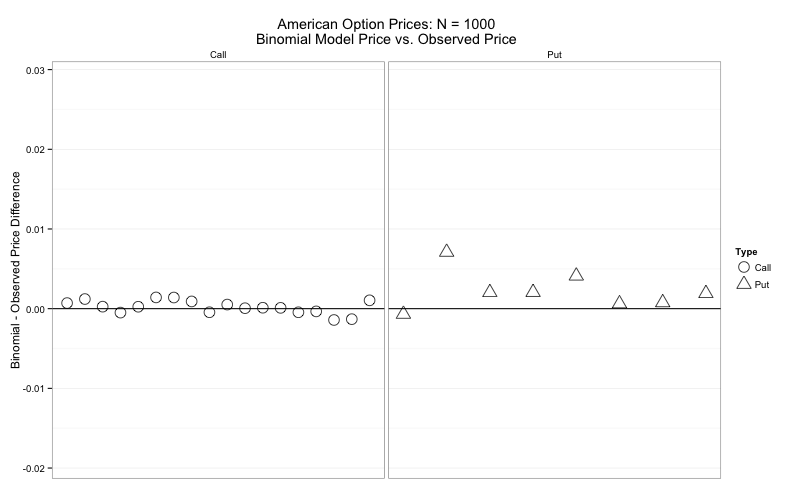
\includegraphics[scale=0.675]{../plots/am_price_diff_N1000.pdf}
 	\includegraphics[scale=0.675]{../plots/am_price_diff_N10000.pdf}
\caption{\footnotesize Price differences between the binomial model and observed market prices given options written on GOOGL over different values of $N = 10^2, 10^3, 10^4$. Implied volatilities for the binomial model computed with $N = 10^5$ and observed market prices.}\label{fig:am_price}
\end{figure}

\indent For $N = 10^2$ we note that the American call option prices computed using the binomial model may be either greater or less than the observed market prices, while American put option binomial model prices are more restricted to being greater than the observed market prices. A pattern emerges when we increase $N$. We find that American call option prices computed by the binomial are approximately equal to the corresponding observed market price, and that American put option prices may be greater than or equal to their corresponding market prices. \\

\indent Note that this pattern aligns with the result from theory stating that the early exercise feature of American call options contribute nothing to its value, that is,
\begin{equation*}
	C^{Am}_0 = C^{Euro}_0
\end{equation*}

while this is not so for American put options. We find, perhaps more intuitively, that the early exercise feature of an American put does indeed make it more valuable, that is
\begin{equation*}
	P^{Am}_0 \geq P^{Euro}_0
\end{equation*}


\newpage
\appendix
\section{Code Output: Data Tables\protect\footnote{Column information: N = number of steps for the binomial model; spots = market closing spot price; strike = contract strike price; tau = years to expiry; ask = market closing ask price; vol = implied volatility via the binomial model; price = American option price via the binomial model using the implied volatility; diff = difference between price and ask, absdiff = absolute difference between price and ask.}}\label{sec:data}
{\small
\csvautolongtable{../data/american_prices_googl_N100.csv}
}
{\small
\csvautolongtable{../data/american_prices_googl_N1000.csv}
}
{\small
\csvautolongtable{../data/american_prices_googl_N10000.csv}
}

\newpage
\section{Code}\label{sec:code}
\subsection{main.cpp}
\lstinputlisting{../code/main.cpp}








\end{document}















